\section{Discussion}

There are a few points to discuss regarding the results found here. The main one is that for every test case but one, the model performed exactly as expected and shows that it is robust and can handle different input values.

The one case that was surprising was the case of varying the center-of-mass energy and observing such a small shift in the $Q$ distributions for the generated events in the hard scattering case. Some investigation into both the code and the physics behind exactly how much the overall center-of-mass energy is related to $Q$ for a given event needs to be done to understand why this happens. Despite the shift being small, I believe it is still significant enough, which is something that was expected of the model, since, despite not knowing exactly how much the ECM should effect $Q$, it is still obvious that it \textit{should}.

Additionally, the lack of comparison to existing data or existing simulation programs has proved completely impossible, not due to the programs being dubbed impossible to use, but because the my program is so specific and other programs include, by default, so many additional processes and features it is immensely difficult to find how to generate results that exactly match the conditions of my program.

Of course, generating some simplistic results with other programs like \textsc{Pythia8} is possible, but completely useless in this case since we'd be comparing apples to oranges. The best that we can do is understand that the model performs qualitatively exactly what is physically expected. What we can do is compare the shapes of the distributions to that generated by a small program written by a computational physicist here at KSU~\cite{PYRESIAS}, which are shown in Figure~\ref{fig:pyresias}. On the left is the $Q$ distribution from the generated events from hard scattering and on the right is the $p_T$ distribution from the generated events from parton showering. Again, the numbers themselves are different so there it is useless to compare there, but we can easily notice that the qualitative behavior of the generated events matches very well.

\begin{figure}[ht]
  \centering
  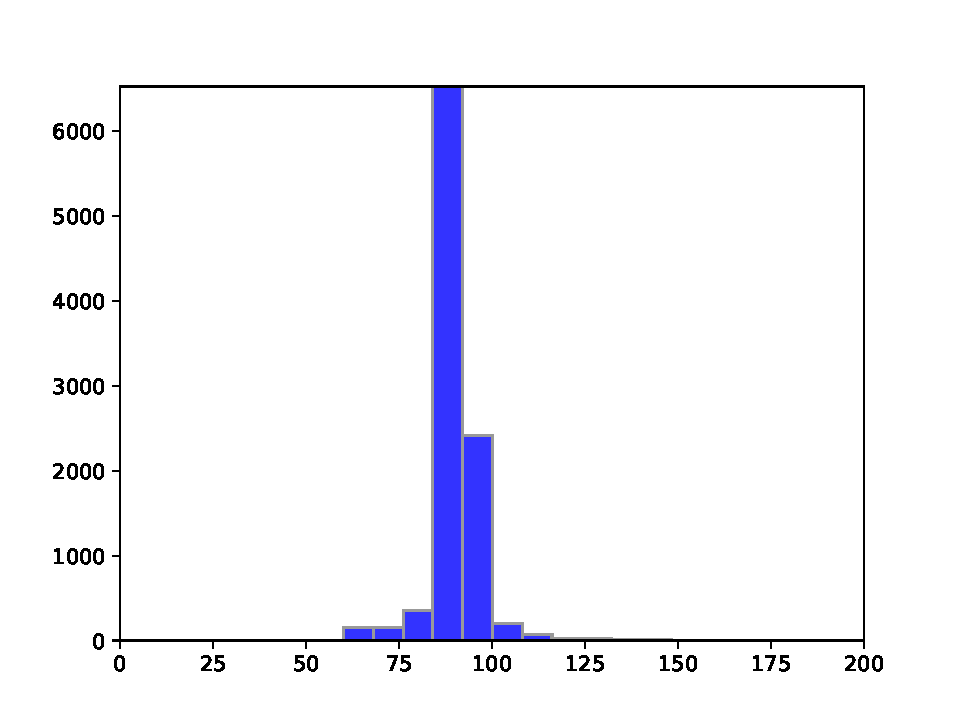
\includegraphics[width=0.45\textwidth]{./res/gfx/Q-pyresias.pdf}
  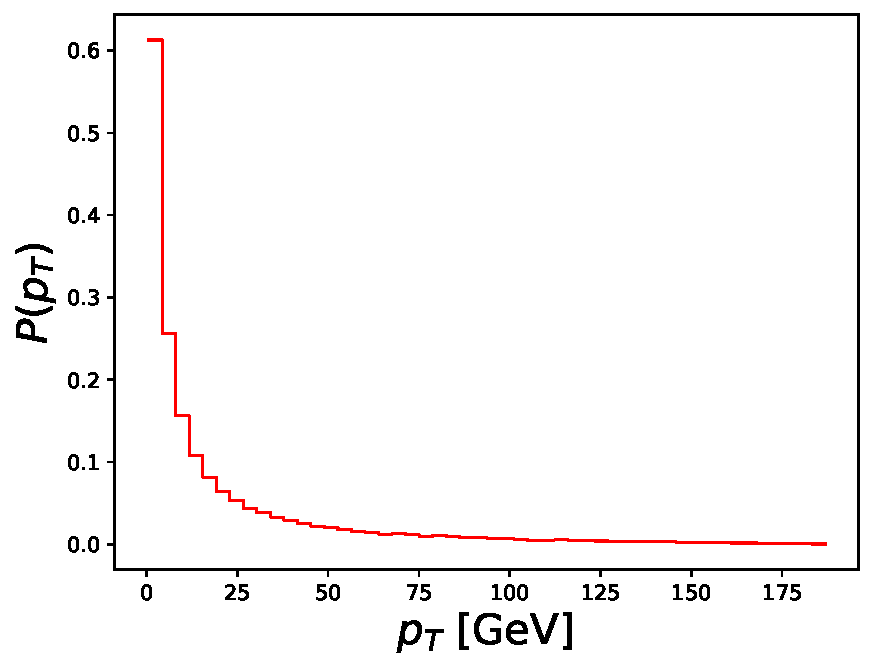
\includegraphics[width=0.45\textwidth]{./res/gfx/pt-pyresias.pdf}
  \caption{$Q$ (left) and $p_T$ (right) distributions from the hard scattering events and parton showering events, respectively, for the toy program \textsc{Pyresias}~\ref{PYRESIAS}.}
  \label{fig:pyresias}
\end{figure}


%%% Local Variables:
%%% mode: LaTeX
%%% TeX-master: "../../Milestone6"
%%% End:
